\documentclass[aspectratio=169]{beamer}

% --------------------------------------------------
% Theme and appearance (matched to aug04.tex)
% --------------------------------------------------

\usetheme{Madrid}
\usecolortheme{default}
\setbeamertemplate{navigation symbols}{}
\setbeamertemplate{caption}[numbered]

\usepackage[T1]{fontenc}
\usepackage{lmodern}
\usepackage{amsmath}
\usepackage{booktabs}
\usepackage{array}
\usepackage{graphicx}
\usepackage{xcolor}

\graphicspath{{../../results/automatic_detector/}
               {../../results/manual_ground_truth/}
               {../../results/pretest/}}

\definecolor{eacolor}{RGB}{230,126,34}
\definecolor{barcodecolor}{RGB}{190,55,55}
\definecolor{normalcolor}{RGB}{55,130,75}
\newcommand{\EA}{\textcolor{eacolor}{\textbf{EA}}}
\newcommand{\Barcode}{\textcolor{barcodecolor}{\textbf{barcoding}}}
\newcommand{\Normal}{\textcolor{normalcolor}{\textbf{normal}}}

\title{Detecting Early Atrophy and Barcoding in OCT}
\subtitle{An Interpretable, Reproducible Image-Analysis Pipeline}
\author{Jonathan Ma}
\institute{Johns Hopkins University}
\date{August 17, 2026}

\begin{document}

\begin{frame}
    \titlepage
\end{frame}

\begin{frame}{The Question We Are Trying to Answer}

An OCT B-scan is a cross-sectional image of the retina. We want to locate and
measure two patterns beneath the retina:

\begin{columns}[T]
\column{0.48\textwidth}
\begin{block}{Early atrophy (EA)}
A broader region with increased transmission of light into deeper tissue.
\end{block}

\column{0.48\textwidth}
\begin{block}{Barcoding}
Repeated vertical bright--dark changes that form a stripe-like pattern.
\end{block}
\end{columns}

\vspace{0.4cm}

The final output is intentionally simple:

\[
\text{each horizontal column}
\longrightarrow
\{\Normal,\ \EA,\ \Barcode\}.
\]

We then report the \textbf{number of detected intervals} and their
\textbf{widths in pixels}. This is exploratory research software, not a
clinically validated diagnostic system.

\end{frame}

\begin{frame}{What Was Built}

The project was reorganized into five independent stages:

\begin{center}
\Large
Loading $\rightarrow$ Preprocessing $\rightarrow$ Detection
$\rightarrow$ Evaluation $\rightarrow$ Visualization
\end{center}

\vspace{0.35cm}

\begin{itemize}
    \item \textbf{Loading:} accepts native HEYEX E2E volumes or PNG + JSON pairs.
    \item \textbf{Preprocessing:} aligns, crops, normalizes, and denoises scans.
    \item \textbf{Detection:} independently identifies EA and barcoding, then
    rejects likely anatomy and vessel shadows.
    \item \textbf{Evaluation:} compares automatic results with manual labels.
    \item \textbf{Visualization:} overlays detections and saves numerical JSON.
\end{itemize}

Each stage has a terminal script with an editable configuration. A separate
validation script runs the complete workflow on all ten selected scans.

\end{frame}

\section{Preprocessing}

\begin{frame}{Why Preprocessing Is Necessary}

Raw OCT scans vary in retinal curvature, brightness, depth, and speckle noise.
The detector should respond to disease patterns rather than these acquisition
differences.

\begin{enumerate}
    \item Use the supplied Bruch's membrane (BM) boundary as a landmark.
    \item Shift each image column so BM becomes horizontal.
    \item Keep the same 150-pixel region beneath BM in every scan.
    \item Put brightness on a comparable scale using z-score normalization.
    \item Apply mild Gaussian denoising while preserving narrow vertical edges.
\end{enumerate}

\begin{center}
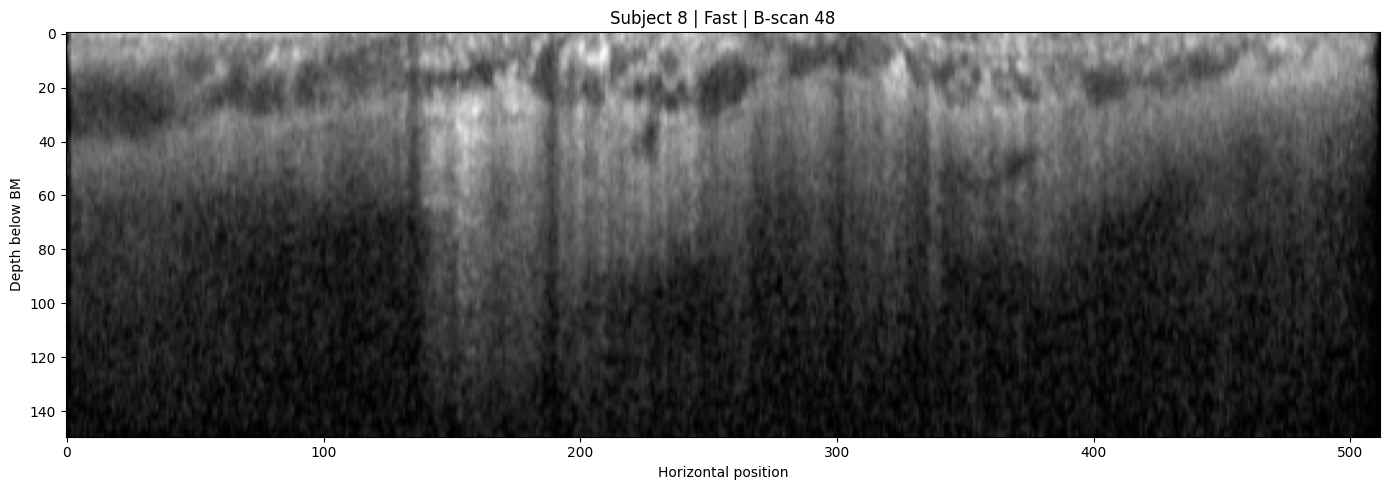
\includegraphics[width=0.68\textwidth]{fast_08_bscan_048_processed.png}
\end{center}

\end{frame}

\begin{frame}{Selected Preprocessing Configuration}

\small
\begin{table}
\centering
\begin{tabular}{>{\raggedright\arraybackslash}p{0.30\textwidth}
                >{\raggedright\arraybackslash}p{0.18\textwidth}
                >{\raggedright\arraybackslash}p{0.43\textwidth}}
\toprule
Setting & Selected value & Plain-language purpose \\
\midrule
Reference layer & BM & Align every scan to the same anatomical boundary. \\
Reference row & Automatic median & Avoid imposing one scanner-specific row. \\
Depth below BM & 150 pixels & Analyze a consistent deep-tissue region. \\
Include boundary & Yes & Retain the BM row at the top of the crop. \\
Require full depth & No & Pad a short crop instead of failing. \\
Normalization & Z-score & Express brightness relative to that scan's mean and spread. \\
Gaussian smoothing & $(1.0,\,0.5)$ & Smooth more through depth than horizontally, preserving stripes. \\
Fill values & 0 & Use the normalized center value for shifted or padded pixels. \\
\bottomrule
\end{tabular}
\end{table}

These settings produced a consistent detector input of approximately
$150\times512$ pixels.

\end{frame}

\begin{frame}{What Normalization and Denoising Mean}

\begin{columns}[T]
\column{0.48\textwidth}
\begin{block}{Z-score normalization}
For every pixel:
\[
Z=\frac{\text{brightness}-\text{scan mean}}
        {\text{scan standard deviation}}.
\]
A value near zero is typical for that scan; a positive value is brighter than
typical. This reduces scan-to-scan brightness differences.
\end{block}

\column{0.48\textwidth}
\begin{block}{Mild Gaussian denoising}
Nearby pixels are gently averaged. The selected strength is greater vertically
($1.0$) than horizontally ($0.5$), reducing granular OCT noise without
smearing the narrow horizontal boundaries of vertical patterns.
\end{block}
\end{columns}

\vspace{0.35cm}

The purpose is not to make the image look prettier. It is to make the same
biological pattern produce more comparable measurements across patients.

\end{frame}

\section{Detector}

\begin{frame}{How the Detector Reads a Scan}

The detector summarizes every horizontal position using four main signals:

\begin{itemize}
    \item \textbf{Typical column brightness:} is the deep tissue broadly bright?
    \item \textbf{Upper brightness:} how bright are the brightest relevant pixels?
    \item \textbf{Depth continuity:} does the pattern persist downward?
    \item \textbf{Vertical organization:} does the texture form organized columns?
\end{itemize}

Each signal is compared with the rest of the same scan using a robust median
and interquartile range. Extreme values are clipped to $[-5,5]$ so a single
artifact cannot dominate the decision.

\vspace{0.3cm}

Eight calibrated inputs are used: the four signals above and four pairwise
interactions. The interactions ask questions such as, ``Is this region both
bright \emph{and} vertically continuous?''

\end{frame}

\begin{frame}{Selected Feature-Extraction Settings}

\scriptsize
\begin{table}
\centering
\begin{tabular}{lcl}
\toprule
Measurement & Value & Plain-language effect \\
\midrule
Verticality smoothing & 1.0 & Reduce speckle before measuring direction. \\
Verticality threshold & 0.60 & Require clear vertical organization. \\
Gradient quantile & 0.80 & Keep the strongest 20\% of local edges. \\
Minimum component size & 0 & Do not remove structures by pixel area here. \\
Column brightness quantile & 0.90 & Summarize the brighter end of each column. \\
Minimum valid pixels & 5 & Avoid estimates based on too few pixels. \\
Column-signal smoothing & 2.0 & Suppress very short horizontal fluctuations. \\
Median / upper IQR multipliers & 1.0 / 0.5 & Set scan-relative brightness requirements. \\
Continuity window / depth lag & 15 / 4 & Test whether structure persists nearby and downward. \\
Continuity quantile & 0.60 & Retain above-typical continuity. \\
Vertical-fraction quantile & 0.70 & Retain the most vertically organized 30\%. \\
Edge margin & 10 columns & Ignore unreliable scan edges. \\
\bottomrule
\end{tabular}
\end{table}

These values create the measurements supplied to the separate calibrated EA,
barcoding, and structural-rejection models.

\end{frame}

\begin{frame}{Separate EA and Barcoding Decisions}

EA and barcoding are not treated as stages of the same rule. Two independently
calibrated models assign a probability to every column:

\begin{columns}[T]
\column{0.47\textwidth}
\begin{block}{Barcoding model}
Selected when probability $\geq 0.55$.

Requires at least 8 consecutive columns and may bridge gaps up to 4 columns.
\end{block}

\column{0.47\textwidth}
\begin{block}{EA model}
Selected when probability $\geq 0.50$.

Requires at least 12 consecutive columns and may bridge gaps up to 5 columns.
\end{block}
\end{columns}

\vspace{0.35cm}

If both models select one column, the detector chooses the class whose
probability is stronger relative to its own threshold. The first and last 10
columns are excluded to reduce edge artifacts.

\end{frame}

\begin{frame}{V3: Requiring Spatial Context}

Earlier versions often selected isolated anatomy that looked disease-like in
one column. V3 requires neighboring evidence.

\scriptsize
\begin{table}
\centering
\begin{tabular}{lccp{0.42\textwidth}}
\toprule
Context setting & Barcoding & EA & Meaning \\
\midrule
Probability smoothing & 2.0 & 2.5 & Look at a small horizontal neighborhood. \\
Weight on original score & 0.65 & 0.60 & Preserve local evidence while adding context. \\
Support radius & 5 & 7 & Check 11 or 15 nearby columns. \\
Minimum nearby support & 55\% & 60\% & Most neighbors must show near-threshold evidence. \\
Required feature votes & 2 of 3 & 3 of 3 & EA uses stricter brightness, continuity, and verticality agreement. \\
Interval mean probability & 0.52 & 0.48 & Reject an entire weak interval. \\
Interval peak probability & 0.68 & 0.62 & Every retained interval needs a convincing core. \\
\bottomrule
\end{tabular}
\end{table}

The less strict barcoding vote was retained because requiring all three
features caused a large loss of true barcoding regions.

\end{frame}

\begin{frame}{Rejecting Vessels and Structural Shadows}

The manual annotations also identify \textbf{uncertain} and
\textbf{vessel/structural} areas. These are excluded from performance scoring;
the detector is not expected to label them as EA or barcoding.

\begin{itemize}
    \item A calibrated structural-rejection model uses 11 intensity and texture
    measurements.
    \item A structural probability of at least $0.90$ activates the veto.
    \item Structural runs must last 3 columns; a 1-column gap may be joined.
    \item The veto expands 2 columns on both sides to cover the shadow boundary.
    \item A second dark-shadow rule requires upper brightness $\leq-1.0$ and
    continuity $\geq0.25$; it expands 3 columns on either side.
\end{itemize}

Disease gap-filling occurs \emph{before} this veto, so rejected structural
columns cannot accidentally be filled back into a disease interval.

\end{frame}

\section{Validation}

\begin{frame}{How the Detector Was Tested}

Ten B-scans were manually annotated, with a different selected scan for each
patient:

\begin{itemize}
    \item five fast-progressing subjects and five slow-progressing subjects;
    \item manual labels for normal, EA, barcoding, uncertain, and structural
    regions;
    \item automatic processing begins from the original E2E volume;
    \item uncertain and vessel/structural columns are ignored during scoring;
    \item EA and barcoding are evaluated separately, one column at a time.
\end{itemize}

\vspace{0.25cm}

This is a useful development set, but it is small and was also used to select
parameters. The reported results measure current fit to these ten scans; they
do not yet demonstrate performance on new patients.

\end{frame}

\begin{frame}{What the Performance Metrics Mean}

\begin{columns}[T]
\column{0.32\textwidth}
\begin{block}{Precision}
Of everything the detector marked, how much was correct?

High precision means fewer false alarms.
\end{block}

\column{0.32\textwidth}
\begin{block}{Recall}
Of all manually marked disease, how much did the detector find?

High recall means fewer missed regions.
\end{block}

\column{0.32\textwidth}
\begin{block}{Dice score}
One summary balancing overlap, false alarms, and misses.

$0$ = no overlap; $1$ = perfect overlap.
\end{block}
\end{columns}

\vspace{0.45cm}

Example: precision of $0.58$ means about 58 of every 100 marked columns were
correct. Recall of $0.52$ means about 52 of every 100 manually marked columns
were recovered.

\end{frame}

\begin{frame}{Best Current Aggregate Results}

\begin{table}
\centering
\begin{tabular}{lcccc}
\toprule
Class & Version & Precision & Recall & Dice \\
\midrule
Barcoding & V2 & 0.526 & 0.506 & 0.516 \\
Barcoding & \textbf{V3 contextual} & \textbf{0.584} & \textbf{0.520} & \textbf{0.550} \\
\midrule
EA & V2 & 0.369 & \textbf{0.739} & 0.492 \\
EA & \textbf{V3 contextual} & \textbf{0.475} & 0.699 & \textbf{0.566} \\
\bottomrule
\end{tabular}
\end{table}

\begin{itemize}
    \item Barcoding false-positive columns decreased from 371 to 302.
    \item EA false-positive columns decreased from 222 to 136.
    \item V3 trades a small amount of EA recall for substantially fewer false
    alarms and better overall overlap.
\end{itemize}

\textbf{Interpretation:} V3 is the best configuration tested so far, but an
aggregate Dice near 0.55 is still development-stage performance.

\end{frame}

\begin{frame}{Examples of Strong Current Results}

\begin{columns}[T]
\column{0.49\textwidth}
\centering

\includegraphics[width=\linewidth]{fast_49_bscan_033_automatic.png}

\small Barcoding: precision 0.930, recall 0.779, Dice 0.848

\column{0.49\textwidth}
\centering

\includegraphics[width=\linewidth]{slow_47_bscan_031_automatic.png}

\small EA: precision 1.000, recall 0.907, Dice 0.951
\end{columns}

\vspace{0.2cm}

Orange denotes EA and red denotes barcoding. These examples show that the
pipeline can closely localize both phenotypes on some scans.

\end{frame}

\begin{frame}{Where the Detector Still Fails}

\begin{columns}[T]
\column{0.49\textwidth}
\centering

\includegraphics[width=\linewidth]{fast_41_bscan_059_automatic.png}

\small Fast 41: unrelated structures survive as high-confidence detections.

\column{0.49\textwidth}
\centering

\includegraphics[width=\linewidth]{slow_17_bscan_055_automatic.png}

\small Slow 17: a disease-negative scan still produces several intervals.
\end{columns}

\vspace{0.2cm}

Spatial cleanup has improved precision, but normal anatomy can still resemble
disease. The next major improvement should be an explicit \textbf{normal
rejection model} using lesion-level depth profiles and independent validation
patients.

\end{frame}

\section{Using the Pipeline}

\begin{frame}{Reproducible Workflow}

After editing the configuration dictionaries in the corresponding scripts:

\begin{enumerate}
    \item Load a selected scan: \texttt{python scripts/load\_data.py}
    \item Preprocess it: \texttt{python scripts/preprocess\_data.py}
    \item Run detection: \texttt{python scripts/run\_detector.py}
    \item Extract interval counts and widths:
    \texttt{python scripts/extract\_numerical\_results.py}
    \item Create an overlay: \texttt{python scripts/visualize\_detector.py}
\end{enumerate}

\vspace{0.3cm}

For the ten annotated scans, one command runs the complete E2E workflow:

\begin{center}
\texttt{python scripts/validation\_test.py}
\end{center}

Outputs use matching names such as
\texttt{fast\_08\_bscan\_048\_automatic.json} and
\texttt{fast\_08\_bscan\_048\_automatic.png}.

\end{frame}

\begin{frame}{Take-Home Messages}

\begin{itemize}
    \item A complete, configuration-driven pipeline now loads, preprocesses,
    detects, measures, evaluates, and visualizes OCT findings.
    \item Consistent BM flattening, a 150-pixel crop, z-score normalization,
    and mild $(1.0,0.5)$ Gaussian denoising are the selected preprocessing
    settings.
    \item EA and barcoding use separate calibrated decisions, spatial context,
    whole-interval confidence, and structural-shadow rejection.
    \item Contextual V3 is the best tested detector: Dice 0.550 for barcoding
    and 0.566 for EA across the ten annotated scans.
    \item Performance varies substantially by patient. More annotations, a
    dedicated normal model, and testing on untouched patients are needed
    before clinical interpretation.
\end{itemize}

\vfill
\centering
\Large Questions?

\end{frame}

\end{document}
